\begin{figure}
    \begingroup
    \setlength{\tabcolsep}{1pt}
    \centering
    \begin{tabular}{@{\hskip 0pt}cc@{\hskip 0pt}cc@{\hskip 0pt}}
    & \smaller{CIFAR-100 (1 Image / Class)} & & \smaller{CIFAR-100 (1 Image / Class)}\\
         \rotatebox[origin=c]{90}{\fontsize{6}{5}\selectfont{$\alpha$: Learned Step Size}} &  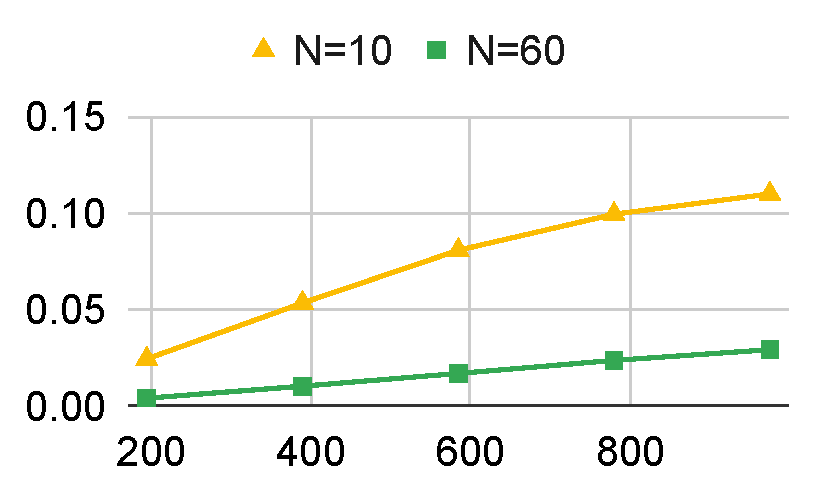
\includegraphics[align=c,width=0.455\linewidth]{figures/learningrate.pdf}& \hfill\;\;\rotatebox[origin=c]{90}{\fontsize{6}{5}\selectfont{Validation Acc. \%}} &  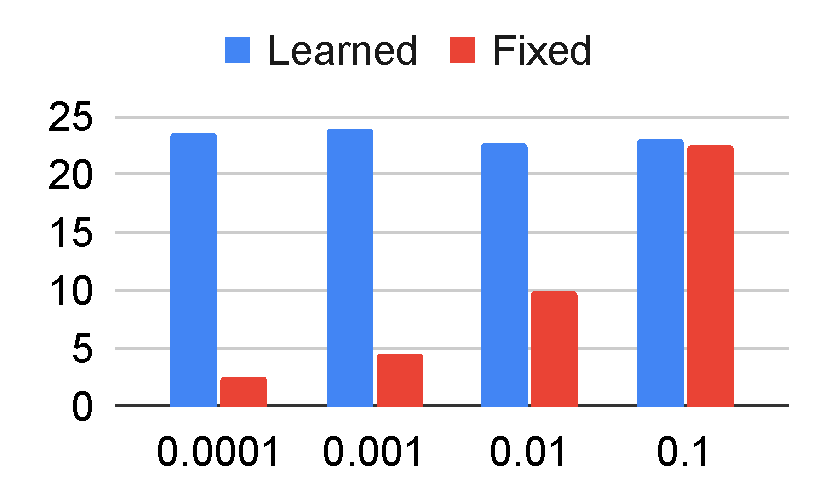
\includegraphics[align=c,width=0.458\linewidth]{figures/lr_lr.pdf}\\[-1.3ex]
         & \fontsize{6}{5}\selectfont{\;\;\;\;\;$M$: Expert Steps} & & \fontsize{6}{5}\selectfont{\;\;$\alpha_0$: Initial Synthetic Step Size}
    \end{tabular}
    \endgroup
        \vspace{-9pt}
    \caption{\textbf{Left:} Our learned synthetic step size $\alpha$ seems to scale inversely with the number of synthetic steps $N$ to cover the same distance in parameter space as the expert steps $M$.
    \textbf{Right:} Having a learnable step size $\alpha$ saves us from having to search for an appropriate fixed $\alpha_0$.
    }
    \lblfig{lr}
    \vspace{-10pt}
\end{figure}